\section{Đọc dữ liệu}
Trước tiên, ta đọc dữ liệu thu từ file "All\_GPUs.csv" và sau đó in ra 3 dòng đầu tiên tương ứng với dữ liệu của mỗi biến. Việc này giúp chúng ta có cái nhìn tổng quan về dữ liệu, hiểu cấu trúc, định hướng trước khi đi sâu vào phân tích. Đồng thời, các giá trị như chuỗi rỗng,\verb|\n|- ", "\verb|\n|", hoặc "\verb|\n|Unknown Release Date" trong file CSV được chuyển thành NA trong data.frame, qua đó giúp chuẩn hóa dữ liệu, tránh các giá trị không hợp lệ và hỗ trợ việc phân tích dữ liệu khuyết sau này.
\begin{minted}{r}
GPU = read.csv("D:/DHBK/HK243/XSTK/BTL/Code_R/All_GPUs.csv",header=TRUE,na.strings = c("","\n-","\n","\nUnknown Release Date"))
head(GPU,3), dim(GPU)
\end{minted}
\textbf{Kết quả:}
\begin{figure}[!h]
    \centering
    \fbox{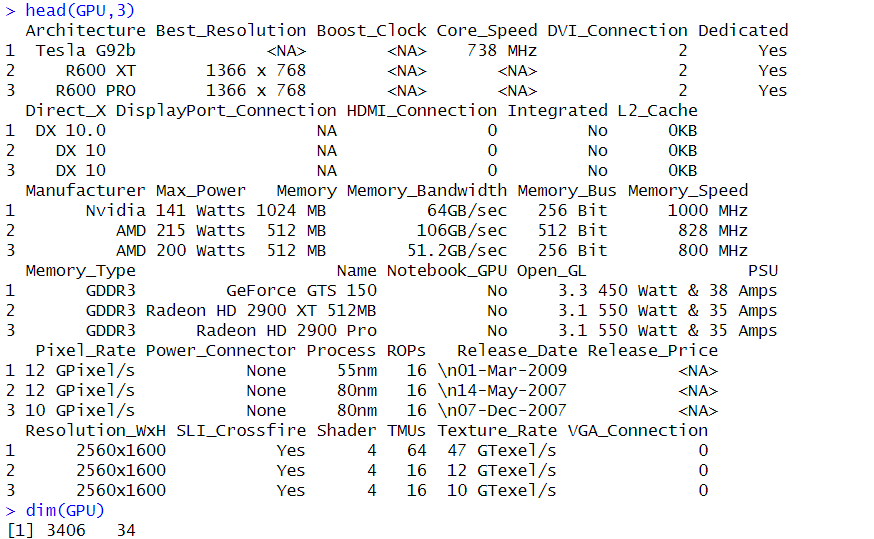
\includegraphics[width=0.75\linewidth]{images/Screenshot 2025-07-29 105142.png}}
    \caption{Các biến có trong dữ liệu ban đầu}
    \label{fig:enter-label}
\end{figure}

\textbf{Nhận xét:}
Kết quả cho thấy, bộ dữ liệu bao gồm 3406 quan sát và 34 biến, tuy nhiên lại có rất nhiều biến chứa dữ liệu khuyết dù chỉ mới xuất ra màn hình 3 dòng đầu. Chính vì thế, việc phân tích dữ liệu khuyết và chọn lọc các biến liên tục và biến phân loại phải được thực hiện một cách hợp lý, tạo tiền đề cho các phân tích chuyên sâu.

\section{Chọn biến và xử lí dữ liệu}
\textbf{a) Cơ sở lựa chọn biến}

Ta thực hiện in bảng thống kê số lượng và tỷ lệ dữ liệu khuyết trong tệp tin bằng các câu lệnh:
\begin{minted}{r}
plot1 <- ggplot(data = na_summary_df, aes(x = reorder(Variable, -Missing), y = Missing)) +
  geom_bar(stat = "identity", fill = "sienna3") +
  geom_text(aes(label = Missing), vjust = -0.5, size = 3) +
  labs(
    title = "Số lượng dữ liệu khuyết theo biến",
    x = "Biến",
    y = "Số lượng dữ liệu NA"
  ) +
  theme_minimal() +
  theme(axis.text.x = element_text(angle = 90, hjust = 1))

plot2 <- ggplot(data = na_summary_df, aes(x = reorder(Variable, -Percentage), y = Percentage)) +
  geom_bar(stat = "identity", fill = "turquoise3") +
  geom_text(aes(label = Percentage), vjust = -0.5, size = 2.5) +
  labs(
    title = "Phần trăm dữ liệu khuyết theo biến",
    x = "Biến",
    y = "Phần trăm dữ liệu NA"
  ) +
  theme_minimal() +
  theme(axis.text.x = element_text(angle = 90, hjust = 1))
plot1 | plot2
ggsave("na_combined_filtered_plot.png", width = 5, height = 12)
\end{minted}

\newpage

\textbf{Ta thu được kết quả như hình 3.2:}
\vspace{0.5cm}
\begin{figure}[!h]
    \centering
    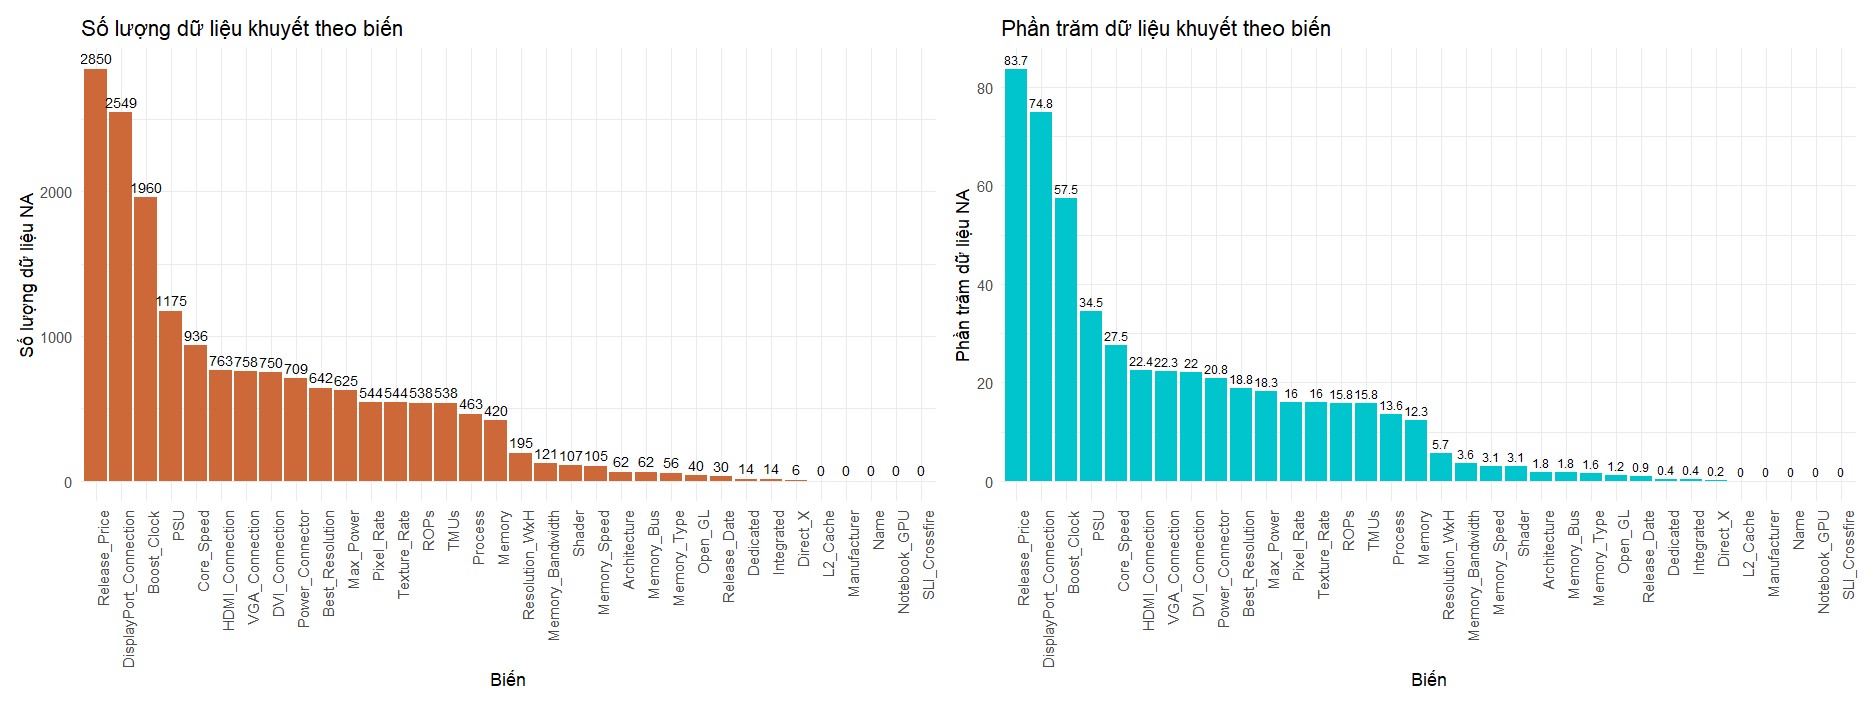
\includegraphics[width=1\linewidth]{images/Rplot01.png}
    \caption{Phân tích dữ liệu khuyết của từng biến trong bộ dữ liệu}
    \label{fig:enter-label}
\end{figure}

\textbf{Nhận xét:}
Ta nhận thấy tỷ lệ dữ liệu khuyết ở các biến có sự khác biệt và chênh lệch nhau lớn. Do đó, đối với những biến có tỷ lệ dữ liệu khuyết cao, ta sẽ không lựa chọn mà chỉ giữ lại các biến có dữ liệu khuyết tương đối.

Qua các cơ sở trên, nhằm tối ưu hóa kết quả khi phân tích hiệu năng GPU máy tính, nhóm quyết định lựa chọn các biến sau:
\colorbox{blue!10}{\hspace{2pt}\textbf{Resolution\_WxH}\hspace{2pt}},
\colorbox{blue!10}{\hspace{2pt}\textbf{Manufacturer}\hspace{2pt}},
\colorbox{blue!10}{\hspace{2pt}\textbf{Core\_Speed}\hspace{2pt}},
\colorbox{blue!10}{\hspace{2pt}\textbf{Memory\_Speed}\hspace{2pt}},
\colorbox{blue!10}{\hspace{2pt}\textbf{Memory\_Type}\hspace{2pt}},
\colorbox{blue!10}
{\hspace{2pt}\textbf{ROPs}\hspace{2pt}},
\colorbox{blue!10}{\hspace{2pt}\textbf{TMUs}\hspace{2pt}},
\colorbox{blue!10}{\hspace{2pt}\textbf{Memory\_Bus}\hspace{2pt}},
\colorbox{blue!10}{\hspace{2pt}\textbf{Memory}\hspace{2pt}},
\colorbox{blue!10}{\hspace{2pt}\textbf{Process}\hspace{2pt}},
\colorbox{blue!10}{\hspace{2pt}\textbf{Shader}\hspace{2pt}},
\colorbox{blue!10}{\hspace{2pt}\textbf{Pixel\_Rate}\hspace{2pt}} (trong đó gồm 3 biến phân loại là
\newline
\colorbox{red!10}{\hspace{2pt}\textbf{Resolution\_WxH}\hspace{2pt}},
\colorbox{red!10}{\hspace{2pt}\textbf{Manufacturer}\hspace{2pt}}, \colorbox{red!10}{\hspace{2pt}\textbf{Memory\_Type}\hspace{2pt}} và 9 biến liên tục) vì các biến này cung cấp cái nhìn toàn diện về hiệu năng GPU, từ sức mạnh xử lý, khả năng kết xuất, đến hiệu quả công nghệ, giúp nhóm đánh giá và so sánh các GPU một cách chi tiết.


% \textbf{1. Resolution\_WxH (Độ phân giải)}

% \begin{itemize}
%     \item \textbf{\textbf{Lý do chọn:}} Độ phân giải tối đa mà GPU hỗ trợ (ví dụ: 1920x1080, 4K, 8K) ảnh hưởng trực tiếp đến khả năng xử lý hình ảnh và đồ họa. GPU có khả năng hỗ trợ độ phân giải cao thường có hiệu năng tốt hơn, đặc biệt trong các ứng dụng như chơi game, chỉnh sửa video, hoặc mô phỏng 3D.
%     \item \textbf{Ý nghĩa:} Biến này giúp đánh giá khả năng hiển thị hình ảnh sắc nét và mượt mà trên các màn hình độ phân giải cao.
% \end{itemize}

% \textbf{2. Manufacturer (Nhà sản xuất)}

% \begin{itemize}
%     \item \textbf{\textbf{Lý do chọn:}} Nhà sản xuất (ví dụ: NVIDIA, AMD, Intel) ảnh hưởng đến chất lượng, độ tin cậy, công nghệ độc quyền (như CUDA của NVIDIA hoặc RDNA của AMD), và hiệu năng tối ưu hóa của GPU. Mỗi nhà sản xuất có các dòng sản phẩm với đặc điểm riêng, phù hợp với các mục đích sử dụng khác nhau (gaming, AI, thiết kế).
%     \item \textbf{Ý nghĩa:} Biến này giúp phân loại GPU theo thương hiệu và so sánh hiệu năng giữa các nhà sản xuất.
% \end{itemize}

% \textbf{3. Boost\_Clock (Tần số tăng tốc)}

% \begin{itemize}
%     \item \textbf{\textbf{Lý do chọn:}} Tần số tăng tốc (Boost Clock, tính bằng MHz hoặc GHz) là tốc độ xung nhịp tối đa mà GPU có thể đạt được khi hoạt động ở chế độ tối ưu. Tần số cao hơn thường tương ứng với hiệu năng xử lý tốt hơn, đặc biệt trong các tác vụ yêu cầu tính toán nhanh.
%     \item \textbf{Ý nghĩa:} Biến này phản ánh sức mạnh xử lý của GPU khi hoạt động ở điều kiện lý tưởng.
% \end{itemize}

% \textbf{4. Core\_Speed (Tốc độ lõi cơ bản)}

% \begin{itemize}
%     \item \textbf{\textbf{Lý do chọn:}} Tốc độ lõi cơ bản (Base Clock) là tốc độ xung nhịp mặc định của GPU. Đây là chỉ số cơ bản để đánh giá hiệu năng ban đầu, trước khi GPU tăng tốc (boost). Sự khác biệt giữa Core Speed và Boost Clock cũng cho thấy khả năng ép xung của GPU.
%     \item \textbf{Ý nghĩa:} Biến này giúp đánh giá hiệu năng cơ bản và tiềm năng tối ưu hóa của GPU.
% \end{itemize}

% \textbf{5. Memory\_Speed (Tốc độ bộ nhớ)}

% \begin{itemize}
%     \item \textbf{\textbf{Lý do chọn:}} Tốc độ bộ nhớ (thường tính bằng MHz hoặc Gbps) quyết định tốc độ truy xuất dữ liệu từ bộ nhớ GPU (VRAM). Tốc độ bộ nhớ cao giúp GPU xử lý nhanh các tác vụ đồ họa phức tạp, như kết xuất hình ảnh hoặc xử lý texture.
%     \item \textbf{Ý nghĩa:} Biến này quan trọng trong việc đánh giá khả năng xử lý dữ liệu đồ họa lớn.
% \end{itemize}

% \textbf{6. Memory\_Type (Loại bộ nhớ)}

% \begin{itemize}
%     \item \textbf{\textbf{Lý do chọn:}} Loại bộ nhớ (ví dụ: GDDR5, GDDR6, HBM2) ảnh hưởng đến băng thông và hiệu suất truyền dữ liệu của GPU. Các loại bộ nhớ mới hơn (như GDDR6X hoặc HBM3) thường cung cấp băng thông cao hơn, cải thiện hiệu năng trong các ứng dụng đồ họa nặng.
%     \item \textbf{Ý nghĩa:} Biến này giúp so sánh hiệu quả của các công nghệ bộ nhớ khác nhau.
% \end{itemize}

% \textbf{7. ROPs (Raster Operation Pipelines)}

% \begin{itemize}
%     \item \textbf{\textbf{Lý do chọn:}} ROPs là các đơn vị xử lý raster hóa, chịu trách nhiệm cho việc kết xuất pixel cuối cùng lên màn hình. Số lượng ROPs cao hơn thường cho phép GPU xử lý nhanh hơn các tác vụ liên quan đến pixel, như chống răng cưa (anti-aliasing) hoặc đổ bóng.
%     \item \textbf{Ý nghĩa:} Biến này quan trọng trong việc đánh giá hiệu năng kết xuất đồ họa.
% \end{itemize}

% \textbf{8. TMUs (Texture Mapping Units)}

% \begin{itemize}
%     \item \textbf{\textbf{Lý do chọn:}} TMUs chịu trách nhiệm ánh xạ texture lên các đối tượng 3D. Số lượng TMUs cao hơn giúp GPU xử lý texture nhanh hơn, cải thiện chất lượng và tốc độ hiển thị trong game hoặc ứng dụng 3D.
%     \item \textbf{Ý nghĩa:} Biến này ảnh hưởng đến hiệu năng trong các tác vụ liên quan đến texture.
% \end{itemize}

% \textbf{9. Memory\_Bus (Độ rộng bus bộ nhớ)}

% \begin{itemize}
%     \item \textbf{\textbf{Lý do chọn:}} Độ rộng bus bộ nhớ (tính bằng bit, ví dụ: 128-bit, 256-bit) quyết định lượng dữ liệu mà GPU có thể truyền từ bộ nhớ trong một chu kỳ. Bus rộng hơn giúp tăng băng thông, cải thiện hiệu năng khi xử lý dữ liệu lớn.
%     \item \textbf{Ý nghĩa:} Biến này quan trọng trong việc đánh giá khả năng truyền dữ liệu của GPU.
% \end{itemize}

% \textbf{10. Memory (Dung lượng bộ nhớ)}

% \begin{itemize}
%     \item \textbf{Lý do chọn:} Dung lượng bộ nhớ (VRAM, tính bằng GB) xác định lượng dữ liệu đồ họa mà GPU có thể lưu trữ. Dung lượng lớn hơn cho phép GPU xử lý các texture lớn, độ phân giải cao, hoặc nhiều tác vụ cùng lúc (như chơi game 4K hoặc học sâu).
%     \item \textbf{Ý nghĩa:} Biến này ảnh hưởng đến hiệu năng trong các ứng dụng đòi hỏi bộ nhớ lớn.
% \end{itemize}

% \textbf{11. Process (Quy trình sản xuất)}

% \begin{itemize}
%     \item \textbf{Lý do chọn:} Quy trình sản xuất (tính bằng nm, ví dụ: 7nm, 5nm) cho biết kích thước bóng bán dẫn trong chip GPU. Quy trình nhỏ hơn thường mang lại hiệu năng cao hơn, tiêu thụ ít điện hơn, và tỏa nhiệt thấp hơn.
%     \item \textbf{Ý nghĩa:} Biến này giúp đánh giá hiệu quả năng lượng và tiềm năng hiệu năng của GPU.
% \end{itemize}

% \textbf{12. Shader (Số lượng đơn vị Shader)}

% \begin{itemize}
%     \item \textbf{Lý do chọn:} Số lượng đơn vị shader (CUDA Cores của NVIDIA hoặc Stream Processors của AMD) quyết định khả năng xử lý song song của GPU. Số lượng shader cao hơn cho phép GPU thực hiện nhiều phép tính đồng thời, cải thiện hiệu năng trong các tác vụ như render 3D hoặc tính toán AI.
%     \item \textbf{Ý nghĩa:} Biến này là chỉ số quan trọng để đánh giá sức mạnh tính toán của GPU.
% \end{itemize}

% \textbf{13. Pixel\_Rate (Tốc độ điền pixel)}

% \begin{itemize}
%     \item \textbf{Lý do chọn:} Tốc độ điền pixel (Pixel Rate, tính bằng GPixel/s) đo lường khả năng GPU vẽ pixel lên màn hình mỗi giây. Pixel Rate cao hơn cho thấy GPU có khả năng xử lý nhanh các tác vụ đồ họa, đặc biệt ở độ phân giải cao.
%     \item \textbf{Ý nghĩa:} Biến này phản ánh hiệu năng kết xuất hình ảnh của GPU.
% \end{itemize}

Câu lệnh thực hiện: 
\begin{minted}{r}
GPU_new = GPU[,c("Resolution_WxH", "Manufacturer", "Core_Speed",
                 "Memory_Speed", "Memory_Type", 
                 "ROPs", "TMUs", "Memory_Bus", "Memory", 
                 "Process", "Shader", "Pixel_Rate")]
\end{minted}

\textbf{b) Xử lí dữ liệu từ các biến đã chọn}

Tiếp theo ta tạo 1 bản tóm tắt thống kê của dataframe của GPU\_new:
\begin{minted}{r}
    print(summary(GPU_new))
\end{minted}

\newpage
\textbf{Kết quả:}
\begin{figure}[!h]
    \centering
    \fbox{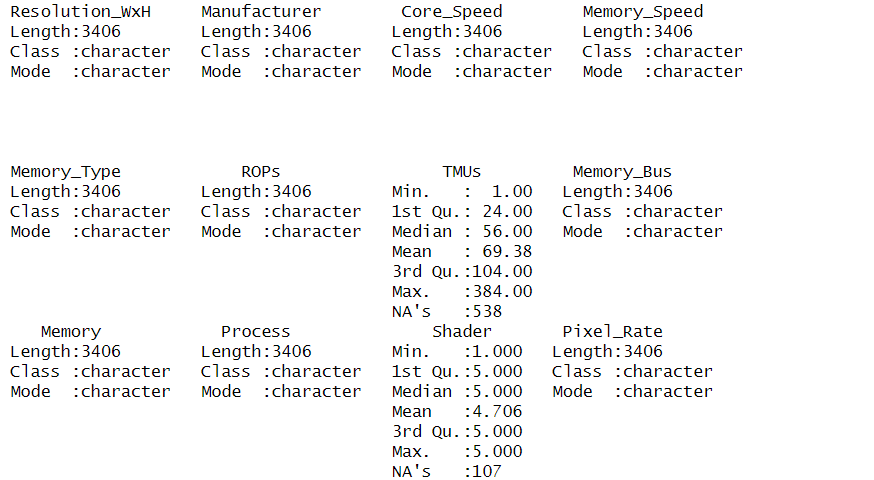
\includegraphics[width=1\linewidth]{images/Screenshot 2025-08-06 231813.png}}
    \caption{Dữ liệu từ dataframe GPU\_new}
    \label{fig:enter-label}
\end{figure}

\textbf{Nhận xét:}

\begin{itemize}
    \item \textbf{Đối với các biến định lượng:}
\end{itemize}

Hầu hết đều ở dạng character (dạng ký tự). Chính vì thế, để có thể phân tích bằng R, ta sẽ chuyển các dữ liệu cần thiết sang số thực. Ta định nghĩa một hàm để tách các đơn vị với chữ số bằng khoảng trắng và chuyển về dạng số thực:
\begin{minted}{r}
helper <- function(x){ 
    if(is.na(x)) return(NA)
    as.double(strsplit(as.character(x), " ")[[1]][1])
}
\end{minted}
Sau đó lần lượt chuyển đổi thành dữ liệu số thực, đồng thời, đối với các dữ liệu khuyết đã chuyển thành NA ban đầu của từng biến, ta thay bằng trung vị của tất cả các dữ liệu trong biến tương ứng:
\begin{minted}{r}   
# Core_Speed
GPU_new$Core_Speed <- sapply(GPU_new$Core_Speed, helper)
GPU_new$Core_Speed[is.na(GPU_new$Core_Speed)] <- median(GPU_new$Core_Speed, na.rm = TRUE)

# Memory_Speed
GPU_new$Memory_Speed <- sapply(GPU_new$Memory_Speed, helper)
GPU_new$Memory_Speed[is.na(GPU_new$Memory_Speed)] <- median(GPU_new$Memory_Speed, na.rm = TRUE)

# ROPs
# Giả sử GPU_new$ROPs đang là character, chứa các giá trị như "24 (x4)", "48 (x2)", v.v. Ta chỉ lấy phần trước dấu ngoặc
GPU_new$ROPs <- as.numeric(sub("^([0-9]+).*", "\\1", GPU_new$ROPs))
GPU_new$ROPs[is.na(GPU_new$ROPs)] <- median(GPU_new$ROPs, na.rm = TRUE)

# TMUs
GPU_new$TMUs <- as.double(GPU_new$TMUs)
GPU_new$TMUs[is.na(GPU_new$TMUs)] <- median(GPU_new$TMUs, na.rm = 
TRUE)

# Memory_Bus
GPU_new$Memory_Bus <- sapply(GPU_new$Memory_Bus, helper)
GPU_new$Memory_Bus[is.na(GPU_new$Memory_Bus)] <- median(GPU_new$Memory_Bus, na.rm = TRUE)

# Memory
GPU_new$Memory <- sapply(GPU_new$Memory, helper)
GPU_new$Memory[is.na(GPU_new$Memory)] <- median(GPU_new$Memory, na.rm = TRUE)


# Process
GPU_new$Process <- as.double(gsub("[^0-9\\.]", "", as.character(GPU_new$Process)))
GPU_new$Process[is.na(GPU_new$Process)] <- median(GPU_new$Process, na.rm = TRUE)

# Shader
GPU_new$Shader <- as.double(GPU_new$Shader)
GPU_new$Shader[is.na(GPU_new$Shader)] <- median(GPU_new$Shader, na.rm = TRUE)

# Pixel_Rate 
GPU_new$Pixel_Rate <- sapply(GPU_new$Pixel_Rate, helper) 
GPU_new$Pixel_Rate[is.na(GPU_new$Pixel_Rate)] <- median(GPU_new$Pixel_Rate, na.rm = TRUE)
\end{minted}

\begin{itemize}
    \item \textbf{Đối với các biến định tính:}
    Ta thay các giá trị khuyết NA thành mode của biến tương ứng. Đồng thời thực hiện chuyển đổi thành factor vì đây là các biến phân nhóm.

\begin{itemize}
    \item \textbf{Resolution\_WxH:}
    Vì giá trị “4096x2160” là mode (giá trị xuất hiện nhiều nhất, chiếm 39\%) nên thay thế các giá trị khuyết bằng giá trị này. Sau đó, chúng ta thực hiện gom nhóm: 4096x2160 (39\%), 2560x1600 (34\%), Other (26\%):
    \begin{minted}{r}
# Resolution_WxH
GPU_new$Resolution_WxH[is.na(GPU_new$Resolution_WxH)] = "4096x2160"
GPU_new$Resolution_WxH <- ifelse(GPU_new$Resolution_WxH == "4096x2160", 1, ifelse(GPU_new$Resolution_WxH == "2560x1600", 2, 3)) # Gom nhóm: 4096x2160 (39%), 2560x1600 (34%), Other (26%)
GPU_new$Resolution_WxH = factor(GPU_new$Resolution_WxH)
    \end{minted}
    \item \textbf{Manufacturer:} 
        \begin{minted}{r}
# Manufacturer
GPU_new$Manufacturer = factor(GPU_new$Manufacturer)
    \end{minted}
    \item  \textbf{Memory\_Type:} Ta xóa các kí tự số và khoảng trống và chỉ giữ lại các kí tự chữ nhằm phân loại tốt hơn:
    \begin{minted}{r}
# Memory_Type
GPU_new <- GPU_new[complete.cases(GPU_new$Memory_Type), ]
GPU_new$Memory_Type = gsub("[^A-Za-z]+.*","",GPU_new$Memory_Type)
GPU_new$Memory_Type = factor(GPU_new$Memory_Type)
    \end{minted}
\end{itemize}
\end{itemize}

\section{Loại bỏ trùng lặp}
Loại bỏ trùng lặp là quá trình loại bỏ các bản ghi hoặc giá trị lặp lại trong một tập dữ liệu để đảm bảo rằng mỗi hàng hoặc giá trị chỉ xuất hiện một lần. Mục đích chính là làm sạch dữ liệu, tránh sai lệch trong phân tích hoặc mô hình hóa do các bản ghi trùng lặp gây ra.

\textbf{1. Ý nghĩa của loại bỏ trùng lặp:}

Nếu một hàng hoặc giá trị xuất hiện nhiều lần (do lỗi nhập liệu, sao chép dữ liệu, v.v.), việc loại bỏ trùng lặp giúp giữ lại chỉ một phiên bản duy nhất. Ngoài ra còn cải thiện độ chính xác bởi trùng lặp có thể làm sai lệch các thống kê (như trung bình, tổng) hoặc làm tăng sai số trong mô hình. Hơn thế, còn có thể giảm kích thước tập dữ liệu, giúp xử lý nhanh hơn.

\textbf{2. Thực hiện trong R:}
Ta sẽ so sánh bộ dữ liệu trước và sau khi đã loại bỏ trùng lặp bằng câu lệnh:
\begin{minted}{r}
    str(GPU_new)
    GPU_new <- dplyr::distinct(GPU_new)
    str(GPU_new)
\end{minted}


\textbf{Kết quả:}
\begin{figure}[!h]
    \centering
    \fbox{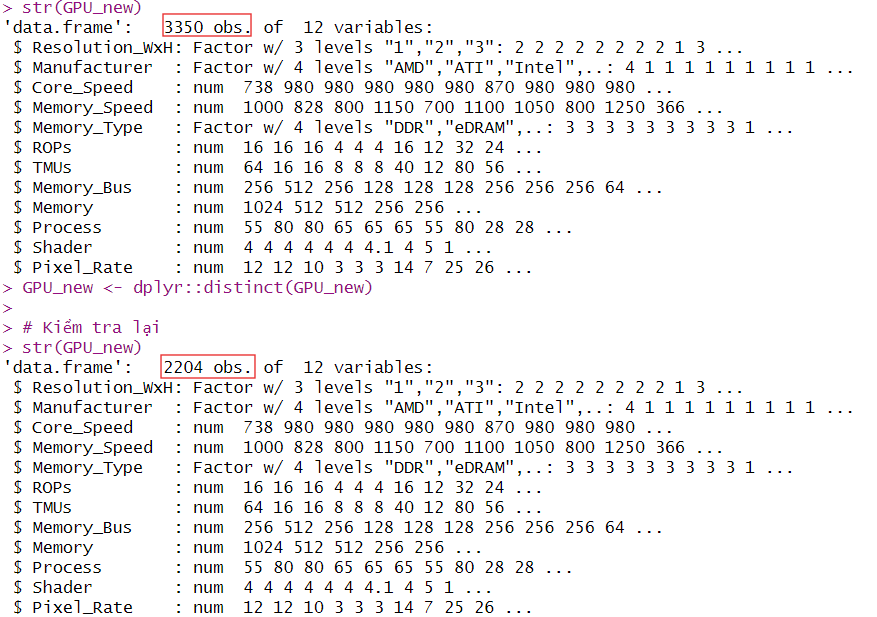
\includegraphics[width=0.9\linewidth]{images/Screenshot 2025-08-06 232835.png}}
    \caption{Hình ảnh đối chiếu trước và sau khi loại bỏ trùng lặp}
    \label{fig:enter-label}
\end{figure}

\textbf{Nhận xét:} Nhận thấy rằng trước khi loại bỏ trùng lặp, tập dữ liệu có tới 3350 quan sát, nhưng sau khi xử lý, số lượng giảm còn 2204. Điều này cho phép cải thiện đáng kể độ chính xác và tối ưu hóa dữ liệu, tạo nền tảng vững chắc để tiến hành các bước phân tích chuyên sâu tiếp theo.



% Ta tạo bảng tóm tắt các cột dữ liệu và tính tổng số giá trị thiếu (NA) trong mỗi cột
% của dataframe GPU\_new sau khi xử lý missing value:
% \begin{minted}{r}
%     print(colSums(is.na(GPU_new)))
% \end{minted}
% \begin{figure}[!h]
%     \centering
%     \fbox{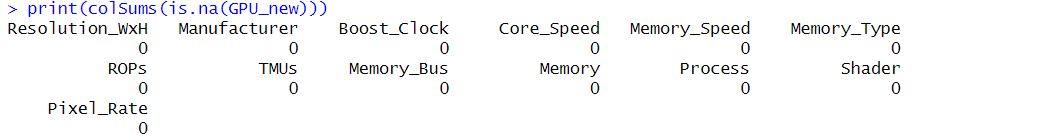
\includegraphics[width=1\linewidth]{images/Screenshot 2025-07-28 172050.png}}
% \end{figure}

% \begin{minted}{r}
%     head(GPU_new,10)
% \end{minted}
% \begin{figure}[!h]
%     \centering
%     \fbox{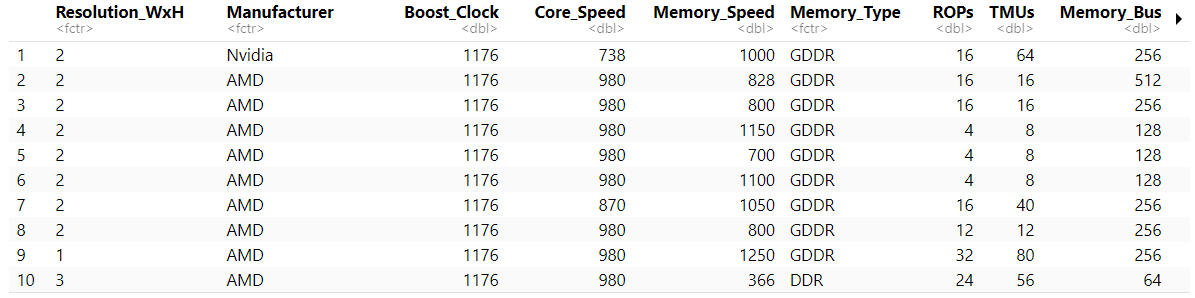
\includegraphics[width=1\linewidth]{images/Screenshot 2025-07-28 172704.png}}
% \end{figure}
% \begin{figure}[!h]
%     \centering
%     \fbox{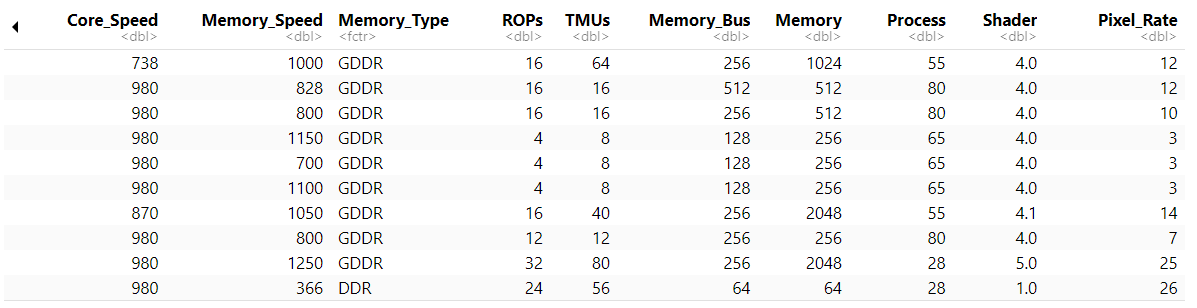
\includegraphics[width=1\linewidth]{images/Screenshot 2025-07-28 172716.png}}
% \end{figure}


% Đến thời điểm này, quá trình tiền xử lý dữ liệu đã hoàn tất thành công, khi các giá trị khuyết thiếu trong bộ dữ liệu đã được xử lý hiệu quả, đồng thời dữ liệu đã được chuẩn bị sơ bộ để sẵn sàng cho các bước thống kê tiếp theo.


\section{Chuyển đổi logarit}
Chuyển dữ liệu sang dạng log: Ta thực hiện đoạn code sau để biến đổi thành dataframe mới tên là GPU\_new\_log. 
\begin{minted}{r}
# Tạo dataframe log-transformed
GPU_new_log <- GPU_new
GPU_new_log[, numerical] <- log(GPU_new_log[, numerical])
GPU_new_log$Pixel_Rate <- log(GPU_new_log$Pixel_Rate)
\end{minted}

\textbf{*Giải thích lý do chuyển sang dạng log}
\begin{itemize}
    \item \textbf{Mối quan hệ phi tuyến tính:} Mối quan hệ giữa biến phụ thuộc và biến độc lập không tuyến tính với nhau, tức là biến độc lập ảnh hưởng đối với biến phụ thuộc không theo cách tuyến tính, mô hình hồi quy thông thường có thể không đáp ứng được. Khi mô hình hồi quy cần mô hình hóa một quan hệ phi tuyến, sử dụng logarit có thể giúp biểu diễn mối quan hệ theo cách linh hoạt và dễ dàng diễn giải.
    \item \textbf{Biến độc lập có biên độ lớn:} Khi biến độc lập có biên độ lớn và tác động không đồng nhất trên biến phụ thuộc, có thể xảy ra hiện tượng hiệu ứng không chính xác hoặc không đồng đều. Bằng cách áp dụng logarit, chúng ta giảm điều lo âu làm cho mô hình trở nên ổn định, đơn giản trong việc diễn giải và tiếp cận.
    \item \textbf{Biến phụ thuộc không tuân theo phân phối chuẩn:} Nếu biến phụ thuộc không tuân theo phân phối chuẩn, điều này có thể ảnh hưởng đến giả định của mô hình hồi quy. Áp dụng logarit có thể giúp làm cho phân phối của biến phụ thuộc gần với phân phối chuẩn hơn, từ đó cải thiện chất lượng của mô hình.
\end{itemize}
Quá trình áp dụng mô hình hồi quy với việc sử dụng logarit đòi hỏi sự cẩn trọng và chặt chẽ. Việc đưa ra quyết định này nên dựa trên quá trình kiểm tra chi tiết và sự hiểu biết sâu sắc về bản chất của dữ liệu. Điều này là chìa khóa quan trọng để đảm bảo rằng mô hình hồi quy không chỉ phản ánh chính xác mối quan hệ giữa các biến mà còn đáp ứng đúng nhu cầu và yêu cầu của vấn đề nghiên cứu.

Kiểm tra lại dữ liệu âm trong dữ liệu gốc và trong dữ liệu sau khi chuyển đổi log-transform:
\begin{minted}{r}
# Kiểm tra xem có giá trị < 0 trong dữ liệu gốc
for (var in numerical) {
    has_negative <- any(GPU_new[[var]] < 0, na.rm = TRUE)
    message(var, " in original < 0? ", has_negative)
}
\end{minted}

\begin{figure}[!h]
    \centering
    \fbox{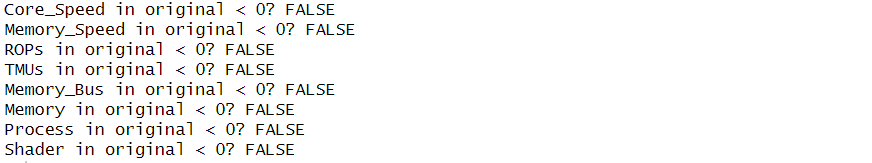
\includegraphics[width=1\linewidth]{images/Screenshot 2025-08-05 153233.png}}
\end{figure}

\begin{minted}{r}
# Kiểm tra xem có giá trị < 0 sau khi log-transform
for (var in numerical) {
 has_negative_log <- any(GPU_new_log[[var]] < 0, na.rm = TRUE)
 message(var, " in log-transformed < 0? ", has_negative_log)
}
\end{minted}

\begin{figure}[!h]
    \centering
    \fbox{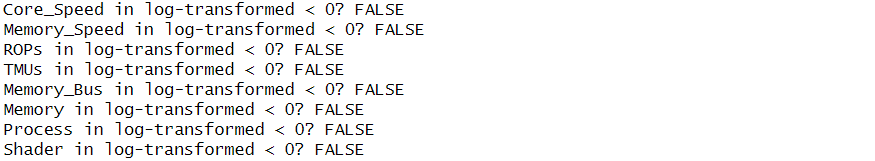
\includegraphics[width=1\linewidth]{images/Screenshot 2025-08-05 153442.png}}
\end{figure}


\section{Tổng kết}

Cuối cùng, ta tạo bảng tóm tắt các cột dữ liệu và tính tổng số giá trị thiếu (NA) trong mỗi cột của dataframe GPU\_new\_log sau khi xử lý missing value.

\begin{minted}{r}
# Thống kê nhanh trên GPU_new_log
print(summary(GPU_new_log))
print(colSums(is.na(GPU_new_log)))
\end{minted}

\begin{figure}[!h]
    \centering
    \fbox{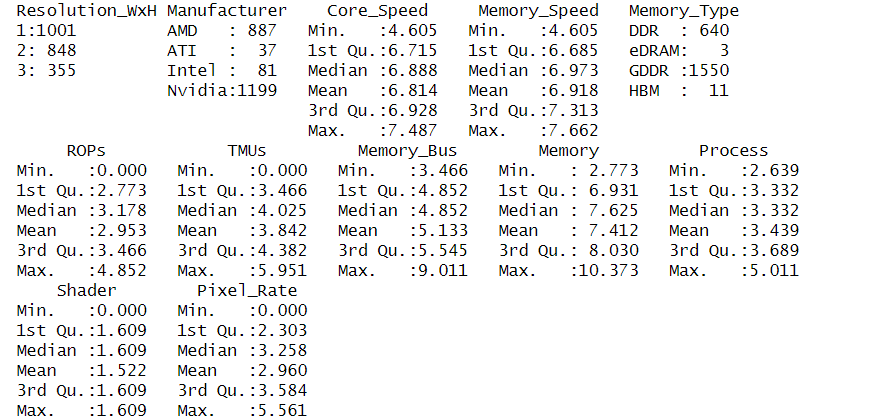
\includegraphics[width=1\linewidth]{images/Screenshot 2025-08-06 233507.png}}
\end{figure}


\begin{figure}[!h]
    \centering
    \fbox{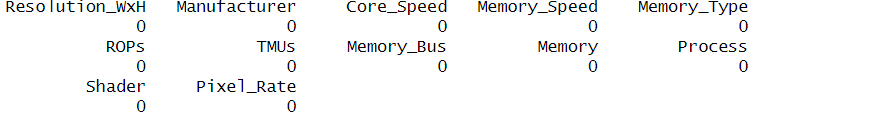
\includegraphics[width=1\linewidth]{images/Screenshot 2025-08-06 233245.png}}
\end{figure}

Đến đây xem như đã hoàn thành việc tiền xử lý số liệu bởi bộ dữ liệu đã được loại bỏ những chỗ bị khuyết cũng như đã được xử lý sơ bộ trước khi tiến hành thống kê. Sau đây, ta sẽ in ra 10 dòng đầu tiên của dataframe GPU\_new\_log. Điều này giúp ta có cái nhìn tổng quan về dữ liệu bằng cách hiển thị một phần của dataframe.

\begin{minted}{r}
# Xem 10 dòng đầu của GPU_new_log
head(GPU_new_log, 10)
\end{minted}

\begin{figure}[!h]
    \centering
    \fbox{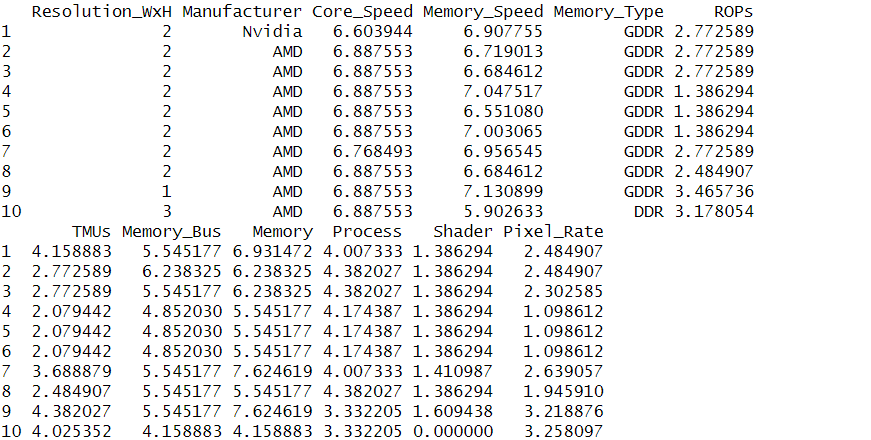
\includegraphics[width=1\linewidth]{images/Screenshot 2025-08-06 233357.png}}
\end{figure}

